\documentclass[a4paper,11pt,twocolumn]{article}

\usepackage{fullpage}
\usepackage[hidelinks]{hyperref}
\usepackage{graphicx}
\usepackage{float}
\usepackage[english]{babel}

\title{\textsc{Team Classified} \\ \small{Sberbank Russian Housing
Market\footnote{\url{https://www.kaggle.com/c/sberbank-russian-housing-market}}}}
\author{Jordi Beernink \and Roel Bouman \and Jeffrey Luppes \and Gerdriaan Mulder \and Thijs Werrij}

\hyphenation{Ada-Boost}

\begin{document}
\maketitle

\section{Introduction}
The \emph{Classified} team worked on the \emph{Sberbank Russian Housing Market}
competition. The competition ran roughly from the start of May until the end of
June, which may shift our final position on the leaderboard. This report gives
insight in the competition, our approach and our results. We discuss our
findings and put forward some critical notes regarding the competition.

\section{Problem description}
Sberbank is the largest, state-owned bank in Russia. They are involved in
financing and brokering deals in the Russian realty market. They
heavily rely on models to predict the value of property. Although the Russian
house market remains fairly stable, the economy relies on natural resources
and is often subject to volatile changes. This makes predicting
property value, whilst correcting for the economy, a non-trivial task.

The goal of the Kaggle competition is to predict realty prices. The dataset
contains training data of 30\,000 properties from 2011 until
2015. The test set is based on entries from 2015 and 2016. Furthermore, a
highly-detailed macro-economic dataset is provided. The true prices of the test
set are not known, and the public leaderboard is based on 35\% of the test data.

The metric used for evaluation on the Kaggle leaderboard is the \emph{Root Mean Squared
Logarithmic Error} (\mbox{RMSLE}). We could submit our predictions five times
per day.

\section{Approach}

We used Apache
Spark\footnote{\url{https://rubigdata.github.io/bigdata-blog-2017-jeffluppes/2017/05/04/Give-me-a-spark/}}
and Python plots to do some early data exploration and visualization. The
JavaScript library ``Leaflet'' was used for plotting data on a map. This method
provided a good early analysis of the data as well as early identification of outliers and
missing data.

\subsection{Exploratory analysis}
The training data was supplied as numerical and categorical data. In order to
work with e.g. a Random Forest Regressor (sklearn) this needed to be one-hot
encoded. For validation purposes, the training set was split in a new training
set containing all entries before 2015, and a validation set consisting of all
entries in 2015. We used internal validation to preliminarily test various
methods. These methods include Linear Regression, Random Forests, AdaBoost, kNN,
XGBoost, Deep Learning and Stochastic Gradient Descent. These methods are easy
to use, readily available, and have been proven to work decently in this domain.

It quickly became clear that eXtreme Gradient Boosting, or XGBoost, outperformed
all other methods. XGBoost outperforms other methods, most likely, by its
inherent ensemble property and by being able to robustly handle different
categories of data. The boosting of weak learners might emphasize the variables
that are useful for prediction, while it de-emphasizes variables that indicate
fraud, thus not modelling unpredictable, fraud-based, outliers.

There was little correlation between internal validation and validation done by
the Kaggle submission platform. It is likely that this is caused by the
presence of fraud in data, which is influential in validation, and may be less
present in the test set. Another explanation might be that there are some
discrepancies in the time-price trend correction, which causes an offset in the
evaluation error. Various forms of validation, including K-fold Cross
Validation, provided no improvement, greatly decreasing the usefulness of
validation. The dataset was far from complete, and many entries were missing
values for variables. It was particularly viable to improve the performance by focusing on
pre-processing.

\subsection{Imputing data}
Various methods of imputing, such as kNN- and SVD-based methods, have been
tested. Matrix Factorization methods, like those used in the famous Netflix
competition, were not readily available, and were too costly to develop
internally. kNN- and SVD-based methods rely on the construction of large
matrices of \emph{sample} $\times$ \emph{sample} size. Those were unfeasible to construct,
because they have an estimated size of over 90\,GB. More memory-efficient
implementations were, again, not available. More simple methods, such as the
mean, modus or median offered no improvement over not replacing the \texttt{NaN}
values in the data. Not replacing the \texttt{NaN} values means some numerical
variables cannot be used for prediction. For categorical variables,
\texttt{NaN} values are treated as a separate category.

\subsection{Regression using XGBoost and Keras}
In the early part of the competition, single models using XGBoost performed
reasonably well, yielding results in the top 20\%. Deep Learning methods using
Keras were not able to compete, and, regardless of network complexity, did not
come close to the performance of single XGBoost models. Deep Learning might
suffer more from a lack of appropriate regularization and an overemphasis of
non-important features. This might be alleviated with more experimentation with
other activation layers or a better batch selection procedure.

Near the end of the competition (and near our project deadline), a modestly
successful kernel was published. This kernel was an ensemble of three XGBoost
models, which, when combined, were able to hit top 5\% at the date of
publication. The bulk of further work was based on these models, being mostly
based on ensemble weighting tweaking. Using linear regression to optimize
ensemble weighting was briefly tested, but was hindered by the little
correlation between validation and testing sets. A graphical representation of
the final model, including the XGBoost parameter settings and other weightings
can be found in appendix~\ref{app:final}.

\section{Results}
The results of some key submissions and models are illustrated in
table~\ref{tbl:xval}. These may not reflect the final position at the end of the
competition. For each implementation, we list details regarding the error
returned by Kaggle. A lower RMSLE score indicates a better performing model. These
results are discussed in depth in the next section.

\begin{table*}[ht]
    \centering
    \begin{tabular}{| p{.25\textwidth} | p{.3\textwidth} | p{.1\textwidth} |
    p{.2\textwidth}|}
    \hline
    \textbf{Classifier} & \textbf{Method} & \textbf{RMSLE} & \textbf{Kaggle Rank
    (of~3077)} \\
    \hline
    XGBoost & Ensemble with 3 models, readjustment of submission & 0.31038 & 146 \\
    \hline
    XGBoost & Ensemble with 3 models & 0.31062 & 266 \\
    \hline
    XGBoost & Single & 0.32575 & 1856 \\
    \hline
    Gradientboosting Regressor & Complete dataset, only 2015 & 0.41384 & 2767 \\
    \hline
    Deep Learning & Dense and Dropout & 0.46745 & 2870 \\
    \hline
    Linear Regression & Complete dataset, only 2015 & 0.49689 & 2897 \\
    \hline
    Decision Tree & Complete dataset, only 2015 & 0.58460 & 3020 \\
    \hline
    SGD Regressor & Naive & 0.59560 & 3021 \\
    \hline
    Benchmark Submission & Naive XGBoost & 0.67333 & 3034 \\
    \hline
    Random Forests & Removing outliers, only 2015 & 0.75239 & 3040 \\
    \hline
    k-Nearest Neighbours & $k = 6$, removing outliers, only 2015 & 0.93122 &
    2050 \\
    \hline
    Random Forest & Naive & 6.12138 & 3072 \\
    \hline
    \end{tabular}
\caption{Overview of key submissions with their models, result and rank}
\label{tbl:xval}
\end{table*}

\section{Discussion}
The ensemble of three XGBoost models performed better than any other method,
including previous XGBoost models individually. Early on in the competition,
these performed with modest success, as they ended up in the middle of the
Kaggle ranking.

The performance of many classic regression methods were poor. The high
complexity and sparsity of the dataset were particularly difficult for these
models, as there are many patterns not identified by linear methods. Still, we
thought these methods could be included in the ensemble, but intermediate
results were not promosing.

The best method was an XGBoost ensemble based on a published kernel by econometrist Andy
Harless\footnote{\url{https://www.kaggle.com/aharless/latest-iteration-in-this-silly-game}},
which included work from other Kaggle contributors. This model was improved
upon, and outperformed the original kernel which, on its own, quickly saw wide
adaption within the community.

The Keras approach (see `Deep Learning' in table~\ref{tbl:xval}), a
10-layer deep neural network could not compete with the success of XGBoost
implementations

In this competition, Kaggle kernels were used with good success. This was very useful as starting point
and inspiration for our own approach(es). We were keeping a close eye on what
the community was coming up with. Some of our code was also published on Kaggle
in the form of kernels.

As we explained earlier, the in-house evaluation method based on the training
data proved to have no correlation with success on the leaderboard. This was the
experience of other Kaggle users as well.

At the moment of writing (20 June 2017) the highest score achieved was 0.31038
with (currently) the rank of 150/3222. This places us in the top 5 percent
(4.65\%, to be exact). The all-time highest placement was rank 49 (top 1.5\%)
with 0.31062 obtained on June 5. Overall, our team made over 50 submissions. If
the competition would end today, we would be awarded silver.

\section{Criticism}
The competition is not without flaws. The test set was very different (both in
balance, and quality) from the training set. This made the evaluation of
candidate submissions non-trivial. Without a proper method of model validation,
we were left in the dark. A lot of data was missing and fraud was suspected in a
significant amount of
objects\footnote{\url{https://www.kaggle.com/c/sberbank-russian-housing-market/discussion/32608}}.

Some major issues were published very late in the competition. Various
details, such as the distance of properties to schools, hospitals and such, were
actually based on the distance to the \emph{housing agencies} instead of the
properties themselves.

\newpage

\onecolumn
\section{Individual contributions}
We started our project with an exploration of the data, in which we all
analyzed the data, generated images and reported our findings in our group
meetings. This free-form allowed us to explore a lot of ideas. After this we
decided how we would tackle the problem: Jordi and Roel looked at
pre-processing, Gerdriaan and Thijs tried different classifiers to see what
worked well, and Jeffrey looked at constructing an ensemble in addition to
standard regression models.

Gerdriaan tested stochastic gradient descent (SGD) and Thijs looked at Keras
Deep Neural Networks, both of which had results that did not look promising
enough to improve on. After discovering the Magic Numbers kernel on Kaggle,
mostly Jordi, Roel and Jeffrey worked at improving this script and making
submissions.

Notes taken at our meetings were written by Jordi. The flash talk was presented
by Jeffrey. To finish the project, we wrote the report together, with editing in
the hands of Jeffrey and Gerdriaan. Gerdriaan worked on the code
delivery\footnote{See our Github repository at
\url{https://github.com/mrngm/Classified} and, more specifically, our final code
(release) at
\url{https://github.com/mrngm/Classified/releases/tag/second\_competition}}.
Thijs and Jeffrey made and presented the final presentation.

\subsection*{Previous competition}
Flashback of the first competition. Pre-processing was done by Jordi and Gerdriaan. The XGBoost implementation was made by Jeffrey and Jordi. Roel made the classification and validation pipeline and worked on Random Forests. Thijs focused on Deep Learning. Jeffrey wrote the report with input from the group. Gerdriaan worked on the code delivery and installed the project on the lilo servers. The first flash talk was done by Roel and the final presentation was made and presented by Gerdriaan and Jordi.

\clearpage

\appendix
\section{The final ensemble method}
\label{app:final}

\begin{figure}[H]
\centering
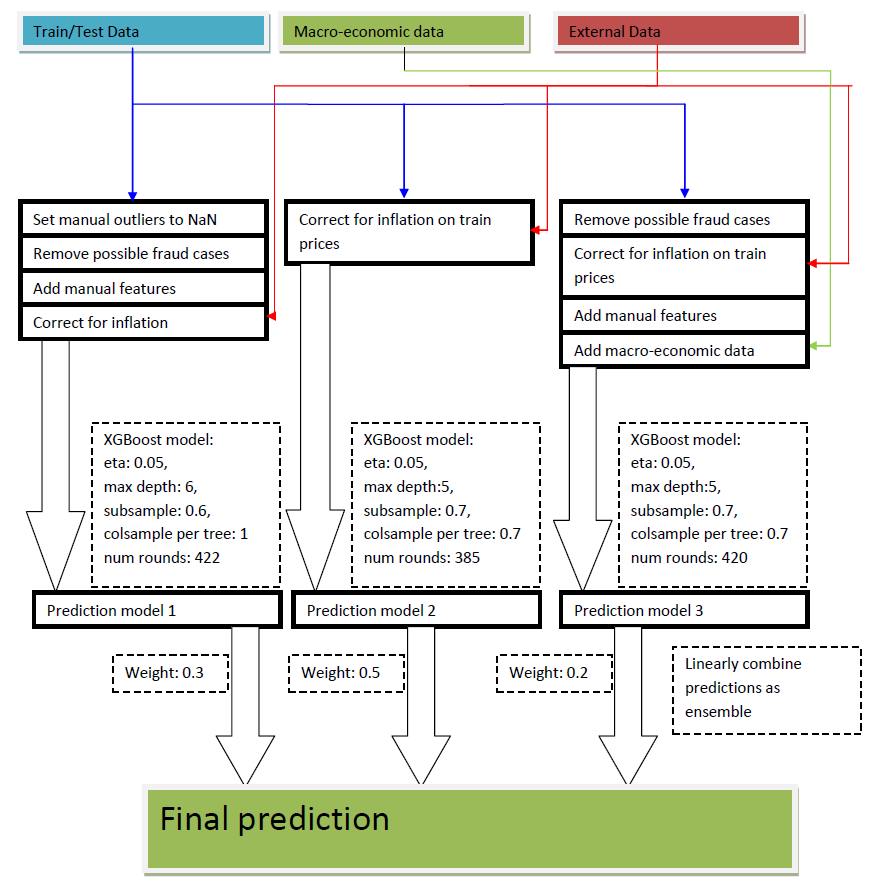
\includegraphics[width=\textwidth]{ensemble.png}
\label{fig:ens}
\end{figure}

The train, test and macro-economic data can be found in train.csv, test.csv and
macro.csv respectively.

Manual outlier detection consisted of detection of data that was incorrect based
on simple logic heuristics. This covers cases such as ``the sum of the area of
the kitchen and living room is larger than the total area'', as well as possible
typo's in for example room number, such as 100 square meter apartments contained
126 rooms.

Some further fraud detection was done by removing extremely high prices from the
training set. A manual selection was made by some Kagglers, based on apartments
selling for 2-5 times the price of regular (identical) apartments.

\end{document}
